{\textbf{1. I/O接口与I/O设备的关系}}

每一台I/O设备都是通过{\textbf{I/O接口}}连接到系统总线上的,并且此总线包括\textbf{数据线、设备选择线、命令线和状态线},如下图所示。

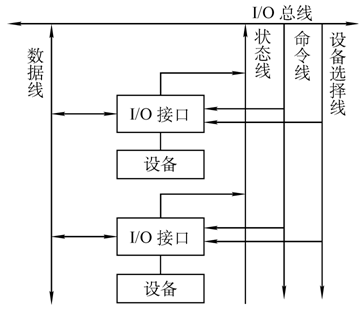
\includegraphics[width=3.33333in,height=2.84375in]{png-jpeg-pics/6A896695497C6EA59B53FA9E705171B6.png}

\textbf{数据线(双向):}用做I/O设备与主机之间传送数据。

\textbf{设备选择线(单向):}用来传送设备码。

\textbf{命令线(单向):}用来传输CPU向设备发出的各种命令信号,如启动、停止、读、写等信号。

\textbf{状态线(单向):}将I/O设备的状态向主机报告的信号线。

{\textbf{2.I/O接口的功能}}

\textbf{(1)选择设备功能}

由于I/O总线与所有设备的接口电路相连,但CPU究竟选择哪台设备,还得通过设备选择线上的设备码来确定,该设备码将送至所有设备的接口,因此当设备选择线上的设备码与本设备码相符合时,应发出设备选择信号SEL,这种功能可通过接口内的设备选择电路来实现。

\textbf{(2)传送命令功能}

当CPU向I/O设备发出命令时,要求I/O设备能作出响应,如果I/O接口不具备传送命令信息的功能,那么设备将无法响应,故通常在I/O接口中设有存放命令的\textbf{命令寄存器和命令译码器}。

\textbf{(3)传送数据功能}

由于I/O接口处于主机和I/O设备之间,因此主机和I/O设备之间\textbf{传送数据必须通过接口}才能实现。这就要求接口中必须具有数据通路,完成数据传送。

\textbf{(4)反映I/O设备的工作状态}

并不是数据发过来就能接收的,因为可能此时还没有准备好,所以接口内必须设置一些反映设备工作状态的触发器。

{\textbf{3.I/O接口的基本结构}}

I/O接口的基本组成如下图所示。

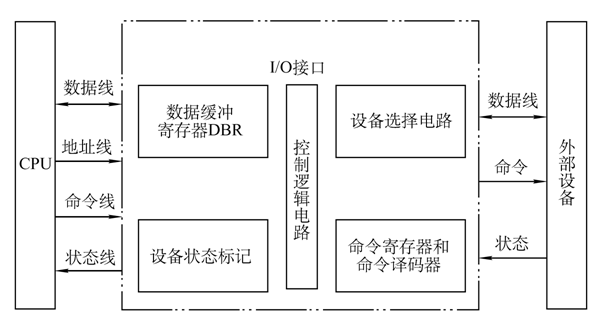
\includegraphics[width=3.33333in,height=1.79167in]{png-jpeg-pics/640D4A2AA720D3DE93F0E3447A74D318.png}

现代计算机一般都采用了\textbf{中断技术},因此接口电路中一般还设有中断请求触发器(INTR),当其为``1''时,表示该I/O设备向CPU发出中断请求。接口内还有屏蔽触发器(MASK),它与中断请求触发器配合使用,完成设备的屏蔽功能。
